\chapter{Estado del Arte}\label{chapter:state-of-the-art}

\section{Interfaz de Usuario}

Los tiempos en que solo los científicos y los desarrolladores de \textit{software} podían usar los ordenadores han quedado muy atrás. Hoy en día, casi todo el mundo puede manejar un PC o una tableta, a menudo incluso sin necesitar conocimientos especializados previos. Esto fue posible gracias al desarrollo de las interfaces gráficas de usuario, un tipo de interfaz de usuario.

\subsection{Orígenes}

Las interfaces de usuario existen desde el surgimiento de las computadoras, incluso mucho antes de que se estableciera el campo de la interacción humano-computadora. A lo largo de los años, han aparecido algunos artículos sobre la historia de la interacción humano-computadora y las interfaces de usuario, centrándose principalmente en la era de la interfaz gráfica y los primeros visionarios como Bush, Engelbart y Kay [\cite{5,6,7,8}].

En las primeras computadoras, la interfaz de usuario consistía en la entrada de una tarjeta perforada o un medio equivalente y, aparte de esta consola operativa, los humanos no tenían interacción con estas primeras computadoras en tiempo real[\cite{6,8}].

Las interfaces de usuario complicadas se consideraron un gasto innecesario porque el \textit{software} fue diseñado para utilizar el procesador al máximo. Esto comenzó a cambiar cuando se introdujeron las interfaces de línea de comandos[\cite{7}], las cuales redujeron en gran medida la latencia a segundos en lugar de días u horas porque la interfaz de usuario era una serie de transacciones de solicitud y respuesta que permitía al usuario cambiar de opinión sobre las transacciones en respuesta a datos en tiempo real de transacciones anteriores.

La siguiente progresión clave de la interfaz de usuario fue la introducción de terminales de visualización de video[\cite{7}]. Hacer que sus entradas de comando aparecieran en una pantalla y poder modificarlas de manera inversa fue mucho más rápido que tenerlas impresas. También tenía sentido desde el punto de vista económico al eliminar la necesidad de tinta y materiales de impresión.

%Finalmente, llegó la GUI, originada principalmente en el Centro de Investigación de Palo Alto (PARC) de Xerox, adoptada y mejorada por Apple y estandarizada efectivamente por Microsoft en sus sistemas operativos Windows.

Luego, en los años 70, los primeros conceptos de interfaz gráfica de usuario se desarrollaron en la empresa Xerox [\cite{5,8}]. Su propósito principal era permitir manejar ordenadores con el ratón y el teclado en lugar de solo con instrucciones en formato de texto. Xerox Alto fue el primer PC con una interfaz gráfica[\cite{7}].

Posteriormente, la llegada de los primeros productos Apple y Microsoft trajo consigo un importante salto adelante en esta materia, tanto así que hoy en día es impensable la interacción con un sistema informático sin este tipo de herramientas virtuales (o naturales) a nuestra disposición[\cite{7,5}].

\subsection{Concepto y características}

Para Moran [\cite{23}], la \textbf{interfaz de usuario} (UI por sus siglas en inglés) consiste en todo lo que el usuario entra en contacto mientras usa el sistema, física, perceptivamente y conceptualmente. La visión conceptual del usuario de la interfaz se desarrolla a partir del comportamiento total del sistema, por lo que la interfaz es más que un componente adicional de una aplicación. Los modelos generalmente aceptados de la interfaz de usuario [\cite{24, 25, 26}] se basan en el modelo de lenguaje de interacción humano-computadora [\cite{28}]. La interacción humano-computadora se considera una forma de comunicación entre dos partes que tienen capacidades de envío y recepción bastante diferentes. Por ejemplo, la computadora tradicionalmente se ha limitado a mostrar mensajes y símbolos en una pantalla. Al mismo tiempo, la computadora también tiene una capacidad bastante limitada para recibir e interpretar información. Por lo tanto, normalmente se requiere que el usuario humano especifique información para la computadora usando teclas en un teclado o clics del mouse.

%La \textbf{interfaz de usuario} (UI por sus siglas en inglés) es el espacio donde se producen las interacciones entre seres humanos y máquinas. El objetivo de esta interacción es permitir el funcionamiento y control más efectivo de la máquina desde la interacción con el humano [\cite{}].

%La tecnología informática permite a las personas interactuar con enormes cantidades de datos utilizando un gran número de funciones. Los comandos de control del usuario y las respuestas de la computadora constituyen una interfaz de usuario, un intercambio de signos gráficos, acústicos y táctiles. En las primeras computadoras interactivas, la interfaz de usuario era la entrada y salida de texto relativamente simple, pero a menudo incómoda. En las interfaces gráficas de usuario actuales, la comunicación se enriquece con computadoras más poderosas, nuevos dispositivos de entrada y salida y software sofisticado. Las interfaces de usuario del mañana se pueden vislumbrar en proyectos de investigación en los que las interfaces de usuario son entornos circundantes que entienden las solicitudes y gestos hablados, y presentan imágenes animadas tridimensionales, videos y agentes autónomos que actúan en nombre del usuario.

El propósito de la interfaz de usuario es facilitar la comunicación entre el usuario y la computadora al envolver el \textit{hardware} y el software, particularmente la semántica de las aplicaciones, en un diálogo. Este diálogo oculta la estructura de los dispositivos de entrada/salida, los sistemas operativos, las redes y las aplicaciones, y permite que el usuario cambie de aplicación rápidamente, sin las trabas de los mecanismos técnicos. Independientemente de cómo evolucione el \textit{hardware} y el software de soporte, la interfaz de usuario permanece incorporada en estos aspectos esenciales: una o más metáforas o ideas subyacentes, la organización conceptual de datos y funciones, técnicas de navegación, características de apariencia y secuencias de interacción [\cite{26}].

La interfaz de usuario se crea en capas de interacción que apelan a los sentidos humanos (vista, tacto, audición y más). Incluyen tanto dispositivos de entrada como teclado, mouse, micrófono, pantalla táctil, escáner de huellas dactilares y cámara, como dispositivos de salida como monitores, parlantes e impresoras. Los dispositivos que interactúan con múltiples sentidos se denominan ``interfaces de usuario multimedia''. Por ejemplo, la interfaz de usuario cotidiana usa una combinación de entrada táctil (teclado y mouse) y una salida visual y auditiva (monitor y parlantes).

Las interfaces de usuario abarcan tres niveles diferentes de interacción entre humano y máquina, que son:

\begin{itemize}
\item Interfaces de hardware: se refieren únicamente a los componentes físicos y electrónicos del sistema que permiten al usuario introducir y extraer información al sistema. Tal es el caso de teclados, ratones (mouse), pantallas táctiles y/o visualizadoras, etc.
\item Interfaces de software, se refieren al funcionamiento específico de los programas informáticos y de la información virtual que ``ocurre'' o ``tiene lugar'' dentro del computador. Tal es el caso de las aplicaciones que empleamos a diario en nuestro trabajo con computadores.
\item Interfaces de software-hardware: se dedican a establecer un puente entre máquina y usuario, para ``traducir'' las instrucciones humanas al lenguaje del sistema y permitirle llevarlas a cabo exactamente, y al mismo tiempo ``traducir'' las respuestas del sistema del código binario a un lenguaje reconocible por el usuario.
\end{itemize}

Al mismo tiempo, de acuerdo a su manera de interactuar con el usuario, las interfaces pueden clasificarse en:

\begin{itemize}
\item Interfaces de línea de comando (CLI, por sus siglas en inglés), cuando consisten en secuencias de caracteres alfanuméricos, es decir, texto únicamente. Por ejemplo, el MS-DOS.
\item Interfaces gráficas de usuario (GUI, por sus siglas en inglés), cuando reproducen un entorno visual simulado (virtual) cuya lógica permite la comunicación con el usuario. Por ejemplo, Microsoft Windows.
\item Interfaces naturales de usuario (NUI, por sus siglas en inglés), cuando emplean dinámicas “naturales” del ser humano, como el habla o el tacto (mediante pantallas táctiles) para comunicarse directamente con el usuario. Por ejemplo, los programas de IA de servicio personal (como Siri, de Apple).
\end{itemize}

%Otros tipos de interfaces de usuario pueden incluir:

%\begin{itemize}
%\item Interfaz de usuario basada en formularios: se utiliza para ingresar datos en un programa o aplicación al ofrecer una selección limitada de opciones. Por ejemplo, un menú de configuración en un dispositivo se basa en un formulario.
%\item Interfaz gráfica de usuario: conocida también como \textbf{GUI} (del inglés \textit{graphical user interface}), es un programa informático que actúa de interfaz de usuario, utilizando un conjunto de imágenes y objetos gráficos para representar la información y acciones disponibles en la interfaz. Su principal uso consiste en proporcionar un entorno visual sencillo para permitir la comunicación con el sistema operativo de una máquina o computador.
%\item Interfaz de línea de comando: en inglés, \textit{command-line interface}, \textbf{CLI}, es un tipo de interfaz de usuario de computadora que permite a los usuarios dar instrucciones a algún programa informático o al sistema operativo por medio de una línea de texto simple
%\item Interfaz de usuario basada en menús: una interfaz de usuario que utiliza una lista de opciones para navegar dentro de un programa o sitio web. Por ejemplo, los cajeros automáticos utilizan interfaces de usuario basadas en menús y son fáciles de usar para cualquier persona.
%\item Interfaz de usuario táctil: Interfaz de usuario mediante háptica o táctil. La mayoría de los teléfonos inteligentes, tabletas y cualquier dispositivo que funcione con una pantalla táctil utilizan la entrada háptica.
%\item Interfaz de usuario de voz: interacciones entre humanos y máquinas mediante comandos auditivos. Los ejemplos incluyen dispositivos de asistente virtual, hablar a texto y GPS.
%\end{itemize}

La interfaz de usuario es importante para cumplir con las expectativas del usuario y respaldar la funcionalidad efectiva de su sitio.  En términos de visibilidad, su diseño y precisión tienen una importancia primordial para representar la cantidad exacta de información para el usuario previsto. Cada decisión menor tomada para el diseño de la interfaz de usuario puede contribuir al software tanto positiva como negativamente.

%Una interfaz de usuario bien ejecutada facilita la interacción efectiva entre el usuario y el programa, la aplicación o la máquina a través de imágenes contrastantes, diseño limpio y capacidad de respuesta.

%La interfaz de usuario (UI) juega un papel vital en el software. En términos de visibilidad, su diseño y precisión tienen una importancia primordial para representar la cantidad exacta de información para el usuario previsto. Cada decisión menor tomada para el diseño de la interfaz de usuario puede contribuir al software tanto positiva como negativamente.

Más específicamente, estos son los elementos generales más importantes de una gran interfaz de usuario:

%\subsection{Elementos generales de la interfaz de usuario}

%Estos son los elementos generales más importantes de una gran interfaz de usuario:
\begin{itemize}
\item Arquitectura de la información (IA por sus siglas en inglés): La funcionalidad de un sitio se construye de acuerdo a la IA. Es importante estructurar y organizar el contenido de su sitio web de forma lógica para ayudar a los usuarios a navegar por el sitio con el mínimo esfuerzo. Los componentes de IA incluyen tres tipos principales de estructuras organizativas: jerárquica (nivel de importancia), secuencial (orden lógico de pasos) y matricial (en la que el usuario elige la organización del contenido que ve).
Ejemplo: elementos de navegación (botones, pestañas, iconos), etiquetas (terminología), funciones de búsqueda (barra de búsqueda) y sistemas de organización (categorías).
\item Diseño interactivo (ID por sus siglas en inglés): los elementos de ID tienen como objetivo convertir a los lectores pasivos en participantes activos al presentar instancias de entrada del usuario. Tener en cuenta al usuario al crear la interfaz de usuario ayudará a mejorar la interactividad y la ejecución de comportamientos específicos que satisfagan las necesidades del usuario. Además, las interfaces de usuario interactivas diseñadas de manera eficiente pueden ``aprender'' a anticipar y solucionar cualquier problema que pueda surgir antes de que afecte negativamente la experiencia del usuario.
Ejemplo: funciones para compartir en redes sociales, conmutadores, botones.
\item Diseño visual: no se puede subestimar la importancia del valor estético de su sitio. El diseño efectivo utiliza elementos de color, contraste, fuente, video y fotografía para atraer a los visitantes y facilitarles la lectura y trabajar con el contenido, en lugar de alrededor de él, para crear un flujo de funcionalidad lógico e intuitivo.
Ejemplo: Contraste, color, espacio en blanco, tipografía, optimización móvil.
\end{itemize}

\subsection{Interfaz de usuario vs experiencia de usuario}

La experiencia de usuario (o \textit{User eXperience}, UX) es la comunicación a través de interfaces, interacción y experiencia que los usuarios tienen con un productos y servicios de la organización [\cite{44}].

A menudo se habla de la interfaz de usuario junto con la experiencia del usuario, que puede incluir la apariencia estética del dispositivo, el tiempo de respuesta y el contenido que se presenta al usuario dentro del contexto de la interfaz de usuario. Ambos términos se incluyen en el concepto de interacción humano-computadora (HCI), que es el campo de estudio que se centra en la creación de tecnología informática y la interacción entre humanos y todas las formas de diseño de tecnología informática[\cite{28}].

Las principales diferencias entre UX y UI son:

\begin{itemize}
\item La UX gira en torno al propósito y la funcionalidad del producto, mientras que la UI se centra en la calidad de la interacción del usuario con el producto.
\item La UX involucra componentes como la investigación de mercado y la identificación de las necesidades del usuario, mientras que la UI tiene componentes de diseño más artísticos relacionados con la apariencia de la experiencia del usuario.
\item La UX se enfoca en la gestión general de proyectos desde la ideación hasta el desarrollo y la entrega, mientras que la UI se enfoca más específicamente en el diseño del producto terminado.
\end{itemize}

\section{Dise\~no de Interfaz de Usuario}

El diseño de interfaz de usuario o ingeniería de la interfaz es el resultado de definir la forma, función, utilidad, ergonomía, imagen de marca y otros aspectos que afectan a la apariencia externa de las interfaces de usuario en sistemas de todo tipo (computadoras de uso general, sistemas de control, dispositivos de comunicación móviles, software de sistemas, software de aplicaciones, sitios web, etc). El objetivo final del diseño de la interfaz de usuario es hacer que la interacción entre el usuario y el sistema del que es interfaz sea tan simple y eficiente como sea posible, en términos de cumplimiento de los objetivos del usuario.

%El objetivo del diseño de una interfaz es producir una interfaz que sea fácil de usar (explicarse por sí misma), eficiente y agradable para que al operar la máquina dé el resultado deseado.

%En general, el objetivo del diseño de la interfaz de usuario es producir una interfaz de usuario que haga que sea fácil, eficiente y agradable (fácil de usar) para operar una máquina de la manera que produce el resultado deseado (es decir, la máxima usabilidad).

En la literatura científica [\cite{35}] sobre el tema en cuestión aparecen principios que regulan los aspectos que deben caracterizar la Interfaz de Usuario como resultado, es decir asociada al producto, sistema de objetos interactivos y visuales que permiten la comunicación entre los usuarios con el sistema informático.

Hay ocho características consideradas al hacer un buen diseño de interfaz de usuario:
\begin{enumerate}
\item Estética: Un buen diseño de interfaz debe ser atractivo. Significa que el uso de esa interfaz es agradable. El diseño debe incluir características interesantes y fáciles de usar con el atractivo visual.
\item Claridad: es la característica más importante del diseño de la interfaz de usuario. El objetivo principal del diseño de la interfaz de usuario es permitir que el usuario interactúe con el sistema comunicándose con él. La interfaz debe evitar la ambigüedad al dejar todo claro a través del lenguaje, la fluidez, la jerarquía y las metáforas de los elementos visuales.
\item Concisión: Es fácil hacer que la interfaz quede clara clarificando y etiquetando todo en exceso, pero esto lleva a que la interfaz se hinche, donde hay demasiadas cosas en la pantalla al mismo tiempo. Si hay demasiadas cosas en la pantalla, es difícil encontrar lo que está buscando y, por lo tanto, la interfaz se vuelve tediosa de usar. El verdadero desafío para hacer una gran interfaz es hacerla concisa y clara al mismo tiempo.
\item Consistencia: Las interfaces coherentes permiten a los usuarios desarrollar patrones de uso. Los usuarios aprenderán cómo se ven los diferentes botones e íconos y los reconocerán y se darán cuenta de lo que hacen en diferentes contextos. Un diseño único con consistencia habla de un buen diseño de interfaz de usuario.
\item Eficiencia: Un buen diseño de interfaz de usuario le permite realizar diferentes funciones de la aplicación de software o sitio web más rápido y con menos esfuerzo.
\item Familiaridad: Incluso si una persona utiliza una interfaz por primera vez, ciertos elementos aún pueden ser familiares. Las metáforas de la vida real se pueden utilizar para comunicar el significado.
\item Perdón: A veces, el usuario comete errores al usar el software o el sitio web. Manejar el error es un indicador importante de la calidad del software. Un buen diseño de interfaz debería permitir al usuario restaurar los elementos eliminados, lo que en un momento u otro se puede hacer sin querer. La interfaz indulgente es una que puede salvar a los usuarios de errores costosos.
\item Capacidad de respuesta (\textit{responsive} en inglés): Una buena interfaz no debe sentirse lenta. Esto significa que la interfaz debe proporcionar buenos comentarios al usuario sobre lo que está sucediendo y si la entrada del usuario se está procesando correctamente.
\end{enumerate}

%En la literatura científica sobre el tema en cuestión aparecen principios que regulan los aspectos que deben caracterizar la Interfaz de Usuario como resultado, es decir asociada al producto, sistema de objetos interactivos y visuales que permiten la comunicación entre los usuarios con el sistema informático. Es muy poco frecuente encontrar reglas, sistemas de principios que normen el proceso de diseño de interfaces con un enfoque integrador, sustentado en la ingeniería de software y en el carácter multidisciplinar y complejo que posee el mismo. 

%Estos principios sustentan el proceso de Diseño de Interfaz de Usuario en cualquiera de las diferentes aplicaciones informáticas que se pueden desarrollar, con cualquiera de las metodologías de la ingeniería de software, dado su carácter flexible y generalizador y se expresan en las cualidades del diseño de interfaz:

%\begin{itemize}
%\item Confiabilidad: apego a las metodologías del proceso de desarrollo de software asociadas al tránsito por todas las fases y flujos de trabajo de este proceso para la elaboración de la interfaz de usuario.
%\item Multidimensional: su conceptualización, diseño, implementación y validación requieren de un análisis desde diferentes dimensiones tecnológicas, semiótico-visuales así como otras específicas de acuerdo al objetivo, tipo y contenido del producto que se desarrolla.
%\item Multidisciplinar: requiere de la intervención de equipos multidisciplinares que aporten criterios para el desarrollo del proceso en consonancia con el producto.
%\item Usabilidad: asociada a la facilidad de uso, la misma se garantiza a través del uso de técnicas de navegación, selección de objetos visuales, diseño de legibilidad, ergonomía, uso de la tipografía, formatos de ficheros adecuados y otros elementos que propician comodidad ante la interacción con la interfaz.
%\item Accesibilidad: el nivel en que logra transmitir a través de los objetos de la interfaz las diferentes funciones, opciones, componentes, tareas, datos e información contentiva. La inteligibilidad y capacidad de emitir mensajes que favorezcan la comprensión de los objetos que estructuran las diferentes pantallas.
%\item Consistencia: está dada en la estabilidad y solidez de la aplicación, la ejecución libre de errores y la respuesta ante cambios de configuración y soporte a través de la interfaz de usuario.
%\item Funcionalidad: funcionamiento óptimo de la aplicación tomando como referencia los requisitos establecidos, los resultados a obtener y las tareas a resolver mediante espacio de interacción entre usuario-dispositivo.
%\item Interactividad: se concreta en los recursos que se emplean para la retroalimentación de la comunicación entre los usuarios con otros usuarios y los dispositivos a través de la interfaz, de forma que favorezcan el intercambio de información, la orientación hacia diferentes tareas, la información del estado del usuario, la aplicación y los datos.
%\item Hipermedialidad: se basa en el uso adecuado de los recursos visuales para transmitir y comunicar la información, aplicación de los principios de la percepción de las formas y configuración de los elementos básicos del diseño, tales como el color, forma, tipografía, agrupamiento por semejanza, proximidad y jerarquía, identidad visual, homogeneidad de las pantallas, relación objeto-fondo e icono-función, uso de los recursos multimedia.
%\item Adaptabilidad: se sustenta en la capacidad de la interfaz de adaptarse a diferentes plataformas y entornos de trabajo aprovechando las potencialidades de los recursos tecnológicos sin afectación en su funcionalidad.
%\end{itemize}

\section{Proceso de diseño de la interfaz de usuario}
El proceso de análisis y diseño de una interfaz de usuario es iterativo y puede representarse mediante un modelo en espiral. El proceso de análisis y diseño de la interfaz de usuario consta de cuatro actividades marco [\cite{36,37}].

\begin{figure}[h]
\centering
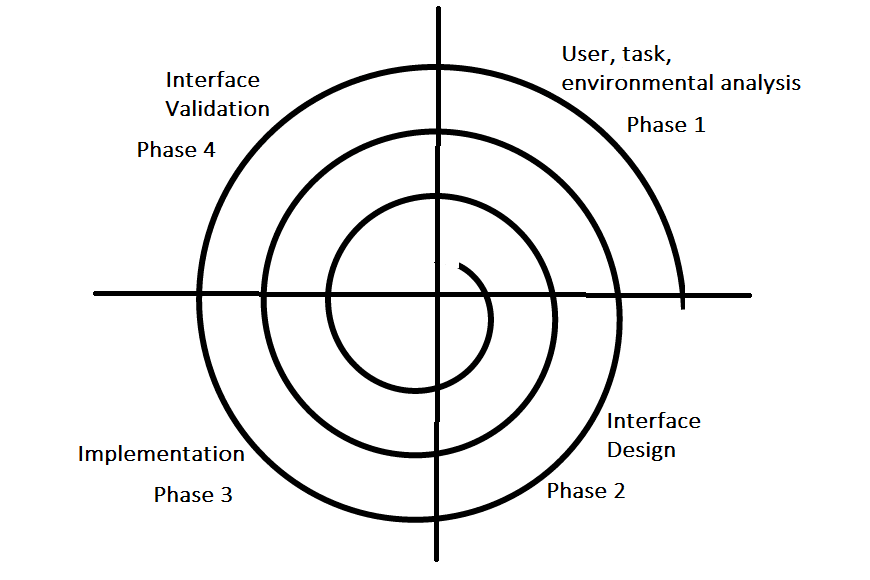
\includegraphics[scale=0.3]{Graphics/espiral}
\caption{Proceso de diseño de interfaz de usuario}
\label{fig:espiral}
\end{figure}

\begin{enumerate}
\item Análisis: El análisis de la interfaz de usuario se centra en el usuario, la tarea, el contenido y el entorno de trabajo que interactúan con el sistema. Inicialmente, el enfoque se basa en el perfil de los usuarios que interactuarán con el sistema, es decir, la comprensión, la habilidad y el conocimiento, el tipo de usuario, etc., según el perfil del usuario, los usuarios se dividen en categorías. De cada categoría se recopilan requisitos. Basado en los requisitos, el desarrollador comprende cómo desarrollar la interfaz. Una vez recopilados todos los requisitos, se realiza un análisis detallado. En la parte de análisis se identifican, describen y elaboran las tareas que realiza el usuario para establecer los objetivos del sistema. El análisis del entorno del usuario se centra en el entorno físico de trabajo.
\item Diseño de la interfaz: el objetivo de esta fase es definir el conjunto de objetos y acciones de la interfaz, es decir, los mecanismos de control que permiten al usuario realizar las tareas deseadas. Indicar cómo estos mecanismos de control afectan al sistema. Especificar la secuencia de acciones de tareas y subtareas, también denominada escenario de usuario. Indicar el estado del sistema cuando el usuario realiza una determinada tarea. Siempre seguir las tres reglas de oro establecidas por Theo Mandel. Los problemas de diseño como el tiempo de respuesta, la estructura de comando y acción, el manejo de errores y las funciones de ayuda se consideran a medida que se refina el modelo de diseño. Esta fase sirve como base para la fase de implementación.
\item Construcción e implementación de la interfaz: La actividad de implementación comienza con la creación de un prototipo (modelo) que permite evaluar escenarios de uso. A medida que continúa el proceso de diseño iterativo, se puede utilizar un conjunto de herramientas de interfaz de usuario que permite la creación de ventanas, menús, interacción de dispositivos, mensajes de error, comandos y muchos otros elementos de un entorno interactivo para completar la construcción de una interfaz.
\item Validación de la interfaz: esta fase se centra en probar la interfaz. La interfaz debería ser tal que debería poder realizar tareas correctamente y debería poder manejar una variedad de tareas. Debe cumplir con todos los requisitos del usuario. Debe ser fácil de usar y fácil de aprender. Los usuarios deben aceptar la interfaz como útil en su trabajo.
\end{enumerate}

Las pruebas determinan la efectividad de una aplicación de interfaz de usuario que debe probarse y expone qué tan fácil o difícil es usar la interfaz de usuario para la audiencia más amplia posible. Los dos principales tipos de pruebas son los siguientes:

\begin{enumerate}
\item Pruebas de usabilidad: evalúan un producto estudiando cómo los usuarios reales realmente usan el sistema. Proporciona una recuperación significativa solo cuando está bien integrado en todo el ciclo de vida del proyecto.
\item Pruebas de accesibilidad: acceden a la aplicación de prueba con tecnologías accesibles y herramientas de prueba automatizadas.
\end{enumerate}

La usabilidad como disciplina constituye un factor determinante de la calidad, cuyo reto es entender cómo los usuarios ven la aplicación web. Por otro lado, la accesibilidad es el grado con que una aplicación web puede ser usada, visitada o accedida por todas las personas independientemente de sus capacidades físicos o técnicas, tema que toma gran importancia para las personas que poseen alguna discapacidad. Ambas disciplinas se encuentran estrechamente relacionadas.

\section{Usabilidad}

En los últimos años, el desarrollo de sistemas interactivos usables y útiles a la vez ha cobrado vital importancia [\cite{1,32}]. Las interfaces de usuario juegan un papel clave en el desarrollo de estos sistemas dado que son las encargadas de  permitir el acceso a los mismos. La usabilidad es un factor clave para el desarrollo de las UI. La usabilidad ha sido definida por la ISO como el grado con que un producto o sistema puede ser usado por usuarios específicos para alcanzar objetivos específicos con efectividad, eficiencia y satisfacción en un contexto de uso dado [\cite{33}]. La dificultad o facilidad que experimenten los usuarios al interactuar con las aplicaciones determinará su éxito o fracaso [\cite{34}]. 

Es importante darse cuenta de que la usabilidad no es una propiedad única y unidimensional de una interfaz de usuario. La usabilidad tiene múltiples componentes y se asocia tradicionalmente con estos cinco atributos [\cite{36}]:

\begin{itemize}
\item Facilidad de aprendizaje: el sistema debe ser fácil de aprender para que el usuario pueda comenzar a trabajar rápidamente con el sistema.
\item Eficiencia: El sistema debe ser eficiente de usar, de modo que una vez que el usuario haya aprendido el sistema, sea posible un alto nivel de productividad.
\item Memorización: el sistema debe ser fácil de recordar, de modo que el usuario ocasional pueda volver al sistema después de un período de no haberlo utilizado, sin tener que aprender todo de nuevo.
\item Errores: El sistema debe tener una tasa de error baja, para que los usuarios cometan pocos errores durante el uso del sistema, y para que si cometen errores, puedan recuperarse fácilmente de ellos. Además, no deben ocurrir errores catastróficos.
\item Satisfacción: El sistema debe ser agradable de usar, de modo que los usuarios estén subjetivamente satisfechos al utilizarlo; les gusta.
\end{itemize}

La usabilidad normalmente se mide haciendo que una cantidad de usuarios de prueba (seleccionados para ser lo más representativos posible de los usuarios previstos) usen el sistema para realizar un conjunto de tareas preespecificado, aunque también se puede medir haciendo que los usuarios reales en el campo realicen las tareas que están haciendo de todos modos. En cualquier caso, un punto importante es que la usabilidad se mide en relación con ciertos usuarios y ciertas tareas.

La usabilidad tiene gran importancia, algunos de sus beneficios son:

\begin{itemize}
\item Una reducción de los costes de producción: los costes y tiempos de desarrollo totales pueden ser reducidos evitando el sobrediseño y reduciendo el número de cambios posteriores requeridos en el producto.
\item Reducción de los costes de mantenimiento y apoyo: los sistemas que son fáciles de usar requieren menos entrenamiento, menos soporte para el usuario y menos mantenimiento.
\item Reducción de los costes de uso: los sistemas que mejor se ajustan a las necesidades del usuario mejoran la productividad y la calidad de las acciones y las decisiones. Los sistemas más fáciles de utilizar reducen el esfuerzo (estrés) y permiten a los trabajadores manejar una variedad más amplia de tareas. Los sistemas difíciles de usar disminuyen la salud, bienestar y motivación y pueden incrementar el absentismo. Tales sistemas suponen pérdidas en los tiempos de uso y no son explotados en su totalidad en la medida en que el usuario pierde interés en el uso de las características avanzadas del sistema, que en algunos casos podrían no utilizarse nunca.
\item Mejora en la calidad del producto: el diseño centrado en el usuario resulta en productos de mayor calidad de uso, más competitivos en un mercado que demanda productos de fácil uso.
\end{itemize}

\section{Accesibilidad}

En la sociedad de la información, las personas acceden a servicios y productos a través de interfaces de usuario. Sin embargo, no todas las personas pueden acceder a ellos, debido a que existen barreras de accesibilidad. Ya no es el caso de que las personas con discapacidad sean los únicos usuarios afectados por las barreras de accesibilidad. De hecho, hoy en día[\cite{39}], numerosos usuarios experimentan problemas a la hora de utilizar la Web, los teléfonos móviles, etc., debido a diferentes tipos de discapacidades, limitaciones funcionales, limitaciones tecnológicas o factores ambientales.

%Para abordar el acceso en este mundo ubicuo, debemos comenzar a pensar en la accesibilidad ubicua y, para algunos, en las interfaces de usuario conectables. La capacidad de "invocar" cualquier tecnología de asistencia o características especiales que se necesiten directamente desde la red para usar en cualquier pantalla que esté cerca, puede ser el medio de acceso más efectivo. Esto es particularmente cierto para las personas que no pueden pagar sus propias tecnologías de la información modernas, sino que confían en las tecnologías que encuentran en los entornos en los que se mueven. Esta capacidad de tener funciones de acceso integradas directamente en la infraestructura que todos usan puede ayudar a nivelar el juego. y, de hecho, significaría que las personas con discapacidad podrían acceder y utilizar las mismas tecnologías principales en los mismos entornos junto con todos los demás.

%La accesibilidad se ha convertido en un tema candente en el diseño web, a pesar de que siempre ha sido parte de la visión original. En un sentido amplio, la accesibilidad simplemente significa garantizar que se pueda acceder a una página determinada en la Web. La accesibilidad no tiene que ver con la discapacidad; más bien, se trata de que las personas accedan a la información compartida que la visión de la Web ha puesto de manifiesto.

%También se ha dicho mucho sobre cómo la accesibilidad se relaciona con los estándares web y viceversa. Siendo realistas, la accesibilidad se basa en aspectos de los estándares web relacionados, pero de hecho se ha convertido en una ciencia, un arte y una práctica propia. Es una especialidad profunda y muy problemática, ya que lo que podría hacer que una página fuera accesible para una persona posiblemente podría volverla inaccesible para otra.

%En informática, la accesibilidad incluye ayudas como las tipografías de alto contraste o gran tamaño, magnificadores de pantalla, lectores y revisores de pantalla, programas de reconocimiento de voz, teclados adaptados, y otros dispositivos apuntadores y de entrada de información.

La accesibilidad aplicada al contenido de Internet se denomina accesibilidad Web. En la Web, el W3C ha desarrollado directrices o pautas específicas para permitir y asegurar este tipo de accesiblidad. El grupo de trabajo dentro del W3C encargado de promoverla es el WAI (\textit{Web Accessibility Initiative}), elaborando para ello unas Pautas de Accesibilidad al contenido Web 1.0, WCAG [\cite{42}].

%Para algunas personas con discapacidades más graves o múltiples, es posible que se necesite una tecnología de interfaz especial que no podría proporcionarse de manera ubicua. Por ejemplo, las personas sordas o ciegas pueden necesitar una pantalla táctil personal. Las personas con discapacidades físicas graves pueden necesitar un transductor de entrada especializado. La capacidad de utilizar estas interfaces alternativas como extensiones naturales de las características ubicuas e integradas permitirá que estas personas también accedan a la Web ya su información. Y la combinación de estos módulos de interfaz personal con software ubicuo y constantemente actualizado puede permitir que estas interfaces especiales funcionen con más y más nuevos tipos de información a medida que evoluciona, aumentando la vida útil de las interfaces y, por lo tanto, reduciendo el costo.

Si bien el acceso a las personas con discapacidad es el enfoque principal de la accesibilidad Web, también beneficia a las personas sin discapacidad. Por ejemplo, un principio clave de la accesibilidad web es diseñar sitios web que sean flexibles para satisfacer las diferentes necesidades de los usuarios. Esta flexibilidad también aumenta la facilidad de uso general y permite que las personas sin discapacidad utilicen los sitios web de acuerdo con sus preferencias, como usar el navegador que deseen y usar atajos de teclado.

Cuando se desarrolla o rediseña un sitio web, la evaluación de la accesibilidad de forma temprana y a lo largo del desarrollo permite encontrar al principio problemas de accesibilidad, cuando es más fácil resolverlos. Técnicas sencillas, como es cambiar la configuración en un buscador, pueden determinar si una página web cumple algunas de las pautas de accesibilidad. Una evaluación exhaustiva, para determinar el cumplimiento de las pautas, es mucho más compleja. 

Hay herramientas de evaluación que ayudan a realizar evaluaciones de accesibilidad. No obstante, ninguna herramienta en sí misma puede determinar si un sitio cumple o no las pautas de accesibilidad. Para determinar si un sitio web es accesible, es necesaria la evaluación humana [\cite{43}].

La accesibilidad de la información basada en la Web se puede mejorar de dos formas principales: mediante el uso de tecnología de acceso y mediante la adopción de buenas prácticas en el diseño de interfaces. Ambos tienen la misma importancia: la provisión de equipos de asistencia (tecnología adaptativa, habilitadora o de acceso) permitirá que un usuario con discapacidad visual acceda a la información en pantalla que recibe la salida de una manera adecuada a sus necesidades. Sin embargo, además de esto, la información proporcionada en pantalla debe presentarse de forma que pueda ser interpretada por cualquier tipo de tecnología de acceso. Esto es lo que se conoce como “diseño web accesible”, “diseño para todos” o “diseño universal”. La necesidad de un enfoque universal ha sido impulsada por la creciente complejidad del diseño y la entrega de información basada en la Web, pasando de una interfaz predominantemente basada en texto a una interfaz multimedia dinámica que ofrece formas visuales, de audio e interactivas. para acceder y utilizar la información proporcionada [\cite{43}].

%Desde un punto de vista técnico, la accesibilidad web es importante para garantizar la interoperabilidad entre diferentes aplicaciones y permitir que los usuarios accedan a la Web utilizando su formato preferido. Esto podría ser a través de tecnología de asistencia para interactuar directamente con el sitio o para descargar información en un formato alternativo.

%Cualquier prueba de accesibilidad debe verse como un proceso que combina herramientas de software automatizadas con juicio humano. No hay ninguna herramienta que pueda ejecutar en su sitio web (o página web, para el caso) para afirmar que es accesible y/o cumple con las disposiciones de la Sección 508 o las Pautas de accesibilidad al contenido web (WCAG)[\cite{43}].

%La interfaz elegida para casi todos los servicios de bibliotecas digitales es la World Wide Web. Aunque se están produciendo cambios significativos en las tecnologías web, la interfaz gráfica de usuario (GUI) se ha convertido rápidamente en la dominante y es probable que siga siéndolo. Desde una perspectiva de accesibilidad, esto ha permitido al menos que se desarrollen enfoques estándar para tratar de garantizar que todos los usuarios puedan acceder a todos los servicios. El sitio web de la biblioteca proporcionará información sobre los horarios de apertura, los servicios ofrecidos y los datos de contacto. También puede ofrecer acceso al catálogo, revistas en línea, resúmenes y páginas de contenido, además de proporcionar acceso en línea a los detalles del prestatario y servicios de renovación y reserva. La provisión de artículos de revistas de texto completo y el desarrollo de la provisión de libros electrónicos brindarán mayores oportunidades para acceder a los servicios de la biblioteca de forma remota. Esto mejorará aún más con la implementación continua de la legislación de derechos de autor que permite que se produzcan formatos alternativos diseñados para personas con discapacidades visuales o de otro tipo a partir de archivos digitales.

\section{Tecnologías empleadas}

Las herramientas de interfaz de usuario han recibido varios nombres a lo largo de los años, siendo el más popular Sistemas de gestión de interfaz de usuario (UIMS). Sin embargo, muchas personas sienten que el término UIMS debe usarse solo para herramientas que manejan la secuencia de operaciones (lo que sucede después de cada evento del usuario), por lo que otros términos como \textit{Toolkits}, Entornos de desarrollo de interfaz de usuario (\textit{User Interface Development Environments}), Constructores de interfaz (\textit{Interface Builders}) y Marcos de aplicación (\textit{Application Frameworks}) también han sido usados [\cite{31}].

Se han diseñado muchos tipos de herramientas para ayudar a crear software de interfaz de usuario, y estos se pueden clasificar por los estilos de las interfaces que crean y las técnicas utilizadas por el diseñador de la interfaz de usuario para crear el software.

%Se han diseñado muchos tipos de herramientas para ayudar a crear software de interfaz de usuario, y estos se pueden clasificar por los estilos de las interfaces que crean y las técnicas utilizadas por el diseñador de la interfaz de usuario para crear el software. Sin embargo, ahora es imposible discutir todas las herramientas de interfaz de usuario, ya que hay muchas. Por ejemplo, hay más de 100 creadores comerciales de interfaces gráficas de usuario, y cada año se informa sobre muchas herramientas de investigación nuevas en conferencias como el Simposio anual de tecnología y software de interfaz de usuario de ACM (UIST) y la conferencia ACM SIGCHI. Por lo tanto, este documento intenta brindar una descripción general de los enfoques más populares, en lugar de una encuesta exhaustiva [\cite{31}].

% En ciencias de la computación, una biblioteca (o library, en idioma inglés) es un conjunto de subprogramas utilizados para desarrollar software. Las bibliotecas de componentes de interfaz de usuario contienen código y datos, que proporcionan servicios a programas independientes, es decir, pasan a formar parte de estos; permitiendo que el código y los datos se compartan y puedan modificarse de formammodular. Algunos programas ejecutables pueden ser a la vez programas independientes y bibliotecas,npero la mayoría de estas no son ejecutables (3).

%Ejecutables y bibliotecas hacen referencias (llamadas enlaces) entre sí a través de un proceso conocido como enlace, que por lo general es realizado por un software denominado enlazador. La mayoría de los sistemas operativos modernos proporcionan bibliotecas que implementan la mayoría de los servicios del sistema. De esta manera, estos servicios se convierten en una "materia prima" que cualquier aplicación moderna espera que el sistema operativo ofrezca. Como tal, la mayor parte del código utilizado por las aplicaciones modernas se ofrece en estas bibliotecas.

%El mundo de la creación de aplicaciones web ha dado pasos agigantados en las últimas décadas. No hace mucho tiempo, clasificar a un trabajador de TI como "desarrollador web" significaba que tenía experiencia en lenguaje de marcado de hipertexto (HTML), hojas de estilo en cascada (CSS) y conocimientos mínimos de JavaScript (JS). Se usó HTML para formatear el contenido y las palabras del sitio web, se usó CSS para hacer que el sitio se viera atractivo con una variedad de colores y diseños y, finalmente, se usó JavaScript para agregar animaciones elegantes en toda la aplicación. Aunque las aplicaciones frontend modernas todavía usan estas tres tecnologías de desarrollo (o lenguajes de desarrollo) en su núcleo, ya no es aceptable simplemente tener un conocimiento "mínimo" de JS. Las demandas de páginas web complejas y completas aumentaron en la esfera del desarrollo frontend, y esto naturalmente resultó en un JavaScript más complejo.

%A medida que aumentaba la complejidad de la cantidad de JavaScript que se incorporaba a la aplicación web, también aumentaba el concepto de lo que significa ser una aplicación web. Los desarrolladores no solo tenían que dar cuenta de la parte frontal de un sitio web, ahora también existe una sección de backend que necesita atención. Aunque no existe una definición de diccionario, una explicación común de lo que se considera backend versus frontend es que “el desarrollo [frontend] es una programación que se enfoca en los elementos visuales de un sitio web o aplicación con los que un usuario interactuará (el lado del cliente). El desarrollo [back-end] se enfoca en el lado de un sitio web que los usuarios no pueden ver (el lado del servidor)”. (Goins, 2020). Cuando las partes de frontend y backend de un sitio web se combinan en una aplicación, la aplicación se considera una aplicación de "pila completa". Las aplicaciones Full Stack requieren más esfuerzo de mantenimiento que las aplicaciones frontend simples, y ahí es donde entran en juego los marcos.

%Desde la aparición de la famosa arquitectura cliente-servidor en la década de los 60, siendo IBM/OS 360 el precursor en esta arquitectura, la misma conforme han pasado los años, se ha desarrollado de manera exponencial, hoy en día los términos front end y back end hacen alusión a esta técnica; siendo el front end el estandarte del cliente mientras que el back end es el estandarte del servidor.

%La construcción de un front end es una tarea delicada dentro de la creación de un proyecto, debido a que no solo puede regirse a los gustos del desarrollador o del cliente, sino también debe regirse a las capacidades técnicas que nos brindan determinadas herramientas de desarrollo. Una página web tradicional se diferencia a una aplicación web porque, la primera hace referencia a una página con información estática no susceptible a la manipulación, mientras, que la aplicación es aquella que se ejecuta en la web así manipulando, procesando presentando y transmitiendo los resultados de manera online, siendo el usuario el que se relaciona directamente con el resultado de ese proceso, denominado producto de información.

Los \textit{frameworks frontends} ofrecen la base para crear y, además, permiten ser flexible respecto a los diseños a implementar. Actualmente, se encuentran una multitud de diferentes \textit{frameworks} con los cuales se pueden realizar un mismo trabajo, aunque cada uno dispone de una curva de aprendizaje distinta, así como sus peculiaridades, conformando diferentes ventajas y desventajas [\cite{48,53}].

En la figura que se muestra a continuación, se puede visualizar cuáles han sido los \textit{frameworks} más de ``moda'' y cómo han ido variando en los últimos años, según el porcentaje de preguntas obtenidas en el famoso dominio ``Stack Overflow''.

\begin{figure}[htp]
\centering
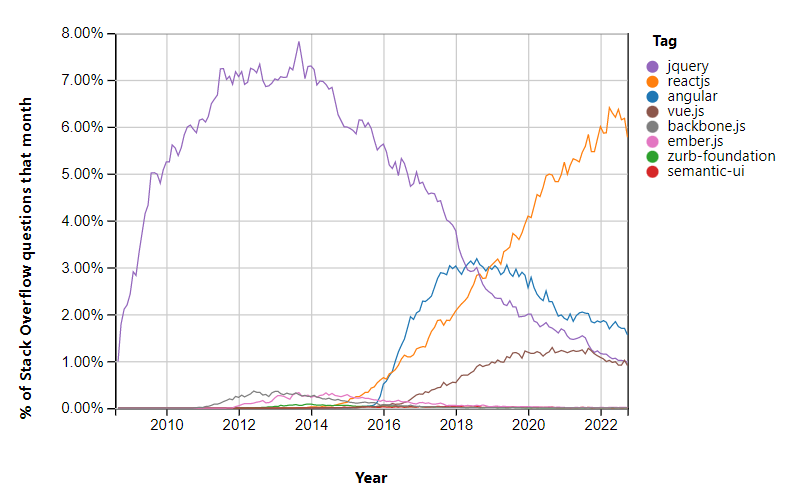
\includegraphics[scale=0.9]{Graphics/stackoverflow}
\caption{Porcentaje de preguntas en Stack Overflow sobre distintos \textit{frameworks}. Fuente:[\cite{50}]}
\label{fig:stackoverflow}
\end{figure}

En la figura anterior, también se observa que, actualmente, los frameworks más usados son React y Angular, sin embargo, Vue se va haciendo un hueco cada vez mayor en la comunidad de interfaces de usuario.

%El desarrollo frontend es un campo que cambia constantemente debido a la gran cantidad de herramientas que se ponen a disposición cada año. Uno de los marcos más populares que se utilizan para crear una experiencia de usuario fluida es el marco Vue. Partiendo del conocido Angular.js, Vue.js es un proyecto independiente de código abierto que está dejando su huella en la comunidad de interfaces de usuario. %51

\subsection{Vue}
%Vue es un framework progresivo JavaScript, esto quiere decir que las principales características, como pueden ser el renderizado y el sistema de componentes, se encuentran ubicadas en una pequeña biblioteca, aunque es posible añadir todas las funcionalidades que se vayan requiriendo según el tipo de proyecto. Algunas de esas características que pueden ser añadidas, que ya traen de partida otros frameworks, son el routing, en el lado del cliente, o manejo de estados mediante vuex o pinia. Esta filosofía permite incluir en la aplicación solo las funcionalidades requeridas.
Vue es un \textit{framework} de JavaScript para construir interfaces de usuario. Se basa en HTML, CSS y JavaScript estándar y proporciona un modelo de programación declarativo y basado en componentes que lo ayuda a desarrollar interfaces de usuario de manera eficiente, ya sean simples o complejas [\cite{47}].

%El principal objetivo que nos encontramos con Vue es la creación de interfaces de usuarios, es por eso por lo que la palabra Vue, es como se denomina a la capa de presentación del modelo MVC (modelo-vista-controlador). El enfoque MVC redujo el uso de recursos de memoria, el tiempo de navegación y la recuperación de datos mediante la reutilización de componentes y la carga parcial del sitio web, obteniendo flexibilidad y comunicación con otras aplicaciones y hardware

Vue es conocido por tener una curva de aprendizaje poco profunda y una implementación progresiva [\cite{49}]. El término framework progresivo por sí mismo es una ventaja, Vue es un \textit{framework} que se puede a aplicar a cualquier proyecto que tenga implementado otras tecnología. También se puede crear proyectos desde cero pensados en escalar su tamaño y sus funcionalidades, como es el caso del sistema que ocupa el tema de esta tesis.

%El manejo de sus componentes, archivos y ficheros, la organización que brinda el entorno de desarrollo para el desarrollador front-end es muy limpia y clara.

El DOM Virtual representa la gran ventaja que Vue cuenta por encima de otro framework [\cite{52}], esta tecnología traída desde React, permite a Vue, no perder tiempo ni rendimiento al cargar todo el árbol de nodos o componentes.

Una de las características, que hace muy cómodo el desarrollo en este \textit{framework}, es que permite dividir las aplicaciones en distintos bloques funcionales independientes llamados componentes, esto se suele denominar arquitectura de componentes. Esta arquitectura permite generar aplicaciones a base de la reutilización de estos componentes, evitando tener código redundante. Además las considerables bibliotecas de componentes de Vue facilitan la reutilización de código, mejoran la productividad del desarrollador y aceleran el proceso de desarrollo.

%Otra de las virtudes de Vue es la capacidad de que las interfaces sean reactivas. Esto significa que se actualiza el HTML y CSS cuando se modifican datos de la aplicación sin que los programadores tengan que realizar una propagación de los cambios de datos de manera manual.

%En cambio, VueJS utiliza el patron Model-View-ViewModel (MVVM) o tambien conocido como Model-View-Whatever. Este patron tiene como objetivo simplificar el desarrollo y el mantenimiento del software. MVVM se divide en 3 partes. Modelo, igual que en otros patrones, representa la capa de datos, contiene la informacion pero nunca la modifica. Vista, su funcion es la de mostrar la informaci ´ on que los usuarios veran. El punto de conexi ´ on entre los 3 componentes comentados anteriormente es el ViewModel o modelo de la vista, donde su funcion es obtener los datos y manipularlos para que se muestren de la forma deseada en la vista. Normalmente hay una ViewModel para cada vista.[7]

%El enfoque Modelo Vista-Controlador redujo el uso de recursos de memoria, el tiempo de navegación y la recuperación de datos mediante la reutilización de componentes y la carga parcial del sitio web, obteniendo flexibilidad y comunicación con otras aplicaciones y hardware

%Las características más importantes de VueJs son:
%• Es un framework progresivo, ya que se puede aplicar a una parte especifica de un aplicativo web
%• Es accesible y escalable
%• Es reactivo, lo que quiere decir tolerante a los fallos
%• Es versátil, ya que el núcleo de VueJs es ligero, y ocupa poco espacio de memoria (74 KB)
%• Tiene una comunidad de programadores que se incrementa, quienes están constantemente mejorando el núcleo.

%Axios es una herramienta familiar en Vue.js porque se usa para mostrar solicitudes AJAX al servicio web. Axios permite crear solicitudes a una URL GET, PUT, POST, DELETE como una API simple, y además posee una biblioteca basada en promesas para recuperar la respuesta con la devolución de llamada [\cite{46}]. 

La herramienta Axios permite crear solicitudes a una URL GET, PUT, POST, DELETE como una API simple, y además posee una biblioteca basada en promesas para recuperar la respuesta con la devolución de llamada. Axios es una herramienta familiar en Vue.js [\cite{46}] lo cual es beneficioso para nuestro sistema que necesita establecer comunicación con el \textit{backend} a través del servicio REST API.
%En la devolución de llamada, se devuelven los datos para la instancia del componente. (Gore 2017).

Vue también brinda una capa de enrutamiento que permite organizar mediante el uso de url, las vistas o componentes se mostrarán en la página, esta capa es fundamental dentro de la seguridad de una aplicación web, ya que permite detener accesos indebidos a vistas destinadas a otros tipos de roles.
Esta capa es muy útil para nuestro sistema que cuenta con distintos roles y permisos para acceder a los datos.

%Aunque Vue está dirigido a aplicaciones de una sola página , también brinda una capa de enrutamiento que permite de mejor manera organizar el contenido en la aplicación. La capa de enrutamiento es aquella, que nos permite organizar mediante el uso de url’s, las vistas o componentes que mostraremos en la página, esta capa es fundamental dentro de la seguridad de una aplicación web, ya que permite detener accesos indebidos a vistas destinadas a otros tipos de roles. peryu

La administración de estado en concepto amplio se refiere a la manera en la que Vue manipula los datos entre componentes estén o no relacionados, generando una especie de almacén donde los componentes podrán acceder para recuperar sus datos [\cite{52}]. 
%La administración de estado en conceptos amplio se refiere a la manera en la que VueJS manipulara los datos entre componentes estén o no relacionados, generando una especie de almacén donde los componentes podrán acceder para recuperar sus datos con respecto a la definición [Vuex busca ayudarnos a lograr una mejor administración del estado imponiendo una tienda centralizada, esencialmente a una sola fuente] (Halliday, 2018).peryu

La persistencia de datos es otra ventaja importante que implementa Vue. Esta función permite que los datos se guarden en el navegador, para que puedan ser usados por los componentes dentro de la vista creada por Vue [\cite{50}]. Añadir la persistencia de datos a nuestro sistema permite optimizar el flujo de las peticiones entre \textit{backend} y \textit{frontend}.

%La persistencia de datos es una pieza clave dentro del rendimiento y la filosofía de desarrollar en VueJS, cualquier aplicación web debe contar con un sistema persistente de datos, para optimizar los flujos de peticiones entre back-end y front-end. peryu

%Gracias a varias características útiles de Vue.js, es una opción preferida para crear muchos sitios web y aplicaciones. Sin embargo, Vue.js se concentra más en la lógica de la aplicación que en su apariencia. Muchos creadores crearon varios marcos de interfaz de usuario de interfaz de usuario para que Vue.js diseñe la interfaz de usuario de manera profesional. Vuetify es uno de estos marcos. Fue creado por John Leider, quien ha trabajado en la comunidad de Vue desde 2014 y cuenta con el respaldo de un vibrante foro de la comunidad de Discord. Vuetify confía en que funcionará en todos los navegadores, incluidos los navegadores antiguos como IE11 y Safari 9 con el requisito de babel-polyfill. Vuetify proporciona varios

%Fortalezas y ventajas de VueJS como herramienta de desarrollo.

%• El termino framework progresivo por sí mismo es una ventaja, VueJS es un framework que se puede a aplicar a cualquier proyecto que tenga implementado otras tecnología, tan solo con importar VueJS traído desde un CDN (Content Delivery Network). También se puede crear proyectos desde cero pensados en escalar su tamaño y sus funcionalidades.

%• No crear nuevas cosas, aunque contradictoriamente el no haber creado nada nuevo, le da una ventaja, puesto que VUEJS logro tomar lo bueno de todas las tecnologías creadas y las transformo en una herramienta más fácil de usar, sin perder robustez.
%• Su entorno para el desarrollo de front-end genera un buen ambiente, sus herramientas son intuitivas y fáciles de usar, obviamente para personas familiarizadas con los conocimientos en el desarrollo front-end.
%• Su reactividad es un framework que se orienta a brindarle a su front–end información constantemente actualizada, bajo esta orientación los desarrolladores solo deben preocuparse en su propósito, generar un buen diseño e una buena interacción con el usuario.
%• El manejo de sus componentes, archivos y ficheros, la organización que brinda el entorno de desarrollo para el desarrollador front-end es muy limpia y clara.
%• Su comunidad, al tener una curva de aprendizaje baja, muchos desarrolladores se suman día a día a esta comunidad desarrollando nuevas herramientas y resolviendo problemas.

%Debilidades y desventajas de VueJS como herramienta de desarrollo.
%
%• La robustez de sus herramientas no oficiales, al ser un framework libre y escalado por la comunidad, sus herramientas complementarias no reciben apoyo de los grandes exponentes en el desarrollo web.
%• El statu quo en el desarrollo de front-end, esta desventaja aunque ajena a la propia herramienta, pone a VueJS fuera de la mira de grandes empresas o proyectos, los desarrolladores tiene una tendencia de mantener las mismas tecnologías.

%En septiembre de 2020, la primera versión de Vue.js, Vue 2, se actualizó a Vue 3. La actualización tuvo un mejor rendimiento general debido a una disminución en el tamaño del código, así como un nuevo formato para manipular la información de la aplicación.

%En cuanto al nivel de presentación se ha elegido el lenguaje Typescript junto con la versión 3 del framework VueJS. VueJS es un framework de javascript que nos permite crear interfaces de manera rápida, escalable y sencilla. Permite desarrollar software de distintas formas, una de ellas es la reactiva, renderizando vistas cuando ocurre un evento, como su rival React. El núcleo de VueJS es muy ligero, convirtiéndolo en un framework muy versátil [35]. En este proyecto se ha trabajado mediante API de composición, lanzada en la versión 3 de Vue, que se centra en funciones de composición, las cuales favorecen la reusabilidad de la lógica entre componentes. Una pieza muy importante es el uso de setup, donde se escribe el código de inicialización del componente a modo de constructor y a su vez se declara el estado reactivo exponiéndolo a la plantilla [36, 14].

Con todo lo expuesto anteriormente, se puede comprobar que Vue es una tecnología que trae beneficios en función de las propiedades deseadas para la interfaz a implementar, pues es liviano, curva de aprendizaje relativamente plana y relativamente fácil de integrar con tecnologías heredadas o una aplicación sin un marco específico. Por estas razones fue el marco de trabajo seleccionado para la solución del problema del presente trabajo.

\subsection{Pinia}

%Hoy en día es necesario hacer uso de alguna librería que nos permita gestionar el estado, almacén de datos compartido por los componentes de la aplicación. La versión 3 de VueJS nos facilita Pinia, librería que gestiona el estado haciendo uso de un store [37]. Un store es un almacén centralizado para mantener los datos que están disponibles, se ha generado uno por cada módulo favoreciendo a la división del código.

Pinia es un nuevo sistema de gestión de estado para Vue [\cite{57}]. Esta es una gran herramienta para cuando se desea compartir datos entre componentes en la aplicación. Una de las razones para usar una herramienta como Pinia (o Vuex para el caso) es que lanzar eventos y escuchar estos eventos en la aplicación puede volverse bastante desordenado y desestructurado. Los sistemas de gestión de estados como Pinia (Vuex, Redux, etc.) pueden ayudar a solucionar esto.

Una gran ventaja de Pinia es su diseño modular, a diferencia de Vuex que proporciona solo una tienda la cual puede tener múltiples módulos dentro de ella, en Pinia se pueden crear varias tiendas que pueden ser importadas directamente a los componentes donde son necesarias[\cite{57}]. Esto permite una mejor división del código y simplifica el desarrollo lo cual es beneficioso para el sistema del presente trabajo.

Pinia tiene soporte integrado para Typescript [\cite{57}], lo cual permite integrar de forma nativa definiciones de tipo dentro de las acciones de Pinia y obtener documentación automática sobre los argumentos que toman las acciones. Además, la seguridad de tipos agrega muchos beneficios a nuestra aplicación, como la prevención de posibles errores de tiempo de ejecución.

Por las razones anteriormente expresadas fue seleccionado Pinia como el sistema de gestión de estados de la aplicación Vue que sera implementada para dar solución al problema de este trabajo.

%Pinia tiene una API más simple que Vuex: La API de Pinia es más simple e intuitiva que Vuex.

%Pinia tiene un diseño modular: Vuex le proporciona una sola tienda que puede tener múltiples módulos dentro de ella. Mientras que en Pinia, puede crear varias tiendas que se pueden importar a componentes directamente donde se necesitan. Esto permite a los empaquetadores dividir mejor el código y proporciona mejores inferencias de TypeScript.
%Tener varias tiendas en lugar de una sola también simplifica el desarrollo, ya que solo se deben usar los métodos de Pinia Store (o módulo) cada vez, en lugar de toda la tienda en Vuex.

%Pinia tiene soporte integrado para Typescript: Lograr que Vuex admitiera tipos siempre había sido una experiencia dolorosa para los desarrolladores de Vue.js. Pinia es una biblioteca de administración de estado completamente tipada que elimina este problema. La seguridad de tipos agrega muchos beneficios a su aplicación, como la prevención de posibles errores de tiempo de ejecución, pero incluso si no está desarrollando su aplicación en TypeScript, obtendrá otros grandes beneficios, gracias a la experiencia de desarrollador rediseñada de Pinia, como la finalización automática. y autosugestión.
%La compatibilidad con TypeScript de Pinia significa que puede hacer cosas como configurar una interfaz para su estado, integrar de forma nativa definiciones de tipo dentro de las acciones de Pinia y obtener documentación automática sobre los argumentos que toman las acciones, completa con autosugerencia y finalización.

%Por estas razones se seleccionó Pinia como el sistema de gestión de estados de la aplicación Vue.js que se implementará para dar solución al problema de este trabajo.

%Pinia se utiliza para guardar el estado de los componentes. Cada vez que se deben enviar datos a la base de datos, se lleva a cabo un determinado procedimiento. Primero, los datos se almacenan temporalmente dentro de la tienda responsable de Pinia y desde dentro de la tienda se activa una llamada API a través de las denominadas acciones. Cada vez que se utiliza Pinia se pueden crear muchas tiendas (Pinia 2022).

\subsection{Typescript}

TypeScript (TS) es un lenguaje de programación desarrollado por Microsoft. TypeScript (TS) es un lenguaje de programación construido a un nivel superior de JavaScript (JS), porque dota al lenguaje de varias características adicionales como el sistema de tipos, el cual nos permite escribir código con menos errores, más sencillo, coherente y fácil de probar [\cite{58, 59}]. 

Los lenguajes de programación tipificados estáticamente están mejor documentados porque el tipado estático en sí mismo actúa como una documentación [\cite{58,60,61}].Esto es una ventaja porque brinda mayor facilidad para otras personas trabajar con nuestro sistema, el cual requiere de posteriores cambios o arreglos a medida que su uso aumente. 

La compatibilidad con TypeScript de Pinia y Vue fueron un factor decisivo para la elección de este lenguaje, además de los ya mencionados beneficios que trae consigo su empleo.
%Esto quiere decir que TypeScript dota al lenguaje de varias características adicionales que hacen que podamos escribir código con menos errores, más sencillo, coherente y fácil de probar, en definitiva, más limpio y sólido [\cite{58, 59}].


%TypeScript agrega escritura estática a JavaScript. [\cite{58, 59}]

%Se informó que los lenguajes de programación tipificados estáticamente están mejor documentados porque el tipado estático en sí mismo actúa como una documentación.[\cite{58}]

%En septiembre del 2020 se liberó lo que conocemos como Vue 3. Todas las novedades de esta nueva versión han relanzado el framework como uno de los más provechosos, obteniendo los desarrolladores una mayor agilidad en su uso. En esta versión todo el framework ha sido implementado bajo TypeScript, el cual ahora se incorpora por defecto en Vue. Esto facilita la reutilización de código y una detección temprana de errores.

%TypeScript (TS) es un lenguaje de programación construido a un nivel superior de JavaScript (JS). Esto quiere decir que TypeScript dota al lenguaje de varias características adicionales que hacen que podamos escribir código con menos errores, más sencillo, coherente y fácil de probar, en definitiva, más limpio y sólido. Algunas ventajas que presenta este lenguaje son las siguientes:

%• Permite usar tipos: esto trae varias ventajas, permite detectar algunos errores en tiempo de diseño sin llegar a la ejecución como pasa con JavaScript, es más fácil entender el código de un vistazo, si se trabaja con algun editor que admita TypeScript se puede detectar errores mientras escribe el código.
%• Es un lenguaje Orientado a Objetos y se pueden usar las características de este: herencia, interfaces, errores tipográficos genéricos, lo que permite un código más ordenado y limpio.
%• Al ser un superconjunto de JavaScript, amplía todas sus funcionalidades, por lo que es compatible con las bibliotecas de JavaScript existentes.

%TypeScript (TS) es un lenguaje increíblemente bien elaborado que respeta y amplía sus raíces de JavaScript. El sistema de tipos parece más expresivo y menos rígido que el de los lenguajes más estáticos y tipificados léxicamente como C$\#$ o Java. Es posible codificar tipos complejos, incluso recursivos, en TypeScript, y se ha demostrado que la sintaxis de definición de tipo es en sí misma Turing-completa. Por estas razones este lenguaje fue seleccionado para la solución del problema de este trabajo.

%Los tipos TS, como cualquier lenguaje escrito, dejan claras sus intenciones, lo que hace que sea mucho más fácil para otras personas trabajar con su código.

\section{REST API}

%La arquitectura orientada a servicios (SOA) se usa generalmente al desarrollar soluciones de software empresarial. Esto brinda flexibilidad para desarrollar diferentes módulos comerciales como servicios allí al brindar escalabilidad y confiabilidad. Entonces la aplicación se acopla débilmente. SOAP y REST son dos enfoques famosos de los servicios web. SOAP (Protocolo simple de acceso a objetos) es un protocolo, mientras que REST (Transferencia de estado representacional) es un estilo arquitectónico en el que se accede a los servicios en forma de Recursos y, en general, se implementan a través de comunicaciones web a través del protocolo HTTP estándar. Los lenguajes de modelado se utilizan para expresar conocimiento/información sobre el sistema que vamos a desarrollar. Para el servicio REST Varios lenguajes/marcos de modelado están presentes en los mundos de la API REST. RAML, Swagger y API Blueprint ahora se usan ampliamente en el desarrollo de API REST.

REST significa transferencia de estado representacional. Este término fue acuñado por primera vez por Roy Fielding[\cite{62}]. REST se refiere al estilo arquitectónico. El estilo arquitectónico REST describe seis restricciones. Estas restricciones, aplicadas a la arquitectura, fueron comunicadas originalmente por Roy Fielding en su tesis doctoral y definen la base del estilo \textit{RESTful}. 

Las restricciones impuestas por la arquitectura REST [\cite{56,62}] son las siguientes:
\begin{itemize}
\item Interfaz uniforme
\item Sin estado
\item Almacenable en caché
\item Cliente-servidor
\item Sistema en capas
\item Código bajo demanda
\end{itemize}

Una REST API describe un conjunto de recursos y un conjunto de operaciones que se pueden llamar en esos recursos [\cite{56}]. La comunicación de la interfaz de usuario de nuestro sistema con el backend se establece mediante un servicio REST API.

%FS 2022-BA-EP-Wisotzki

%Aunque no hubo regulaciones estrictas sobre las tecnologías utilizadas, se sugirió enfáticamente trabajar con tecnologías ya presentes dentro del departamento y el equipo asesor. Además, el cliente también tenía que estar familiarizado con el desarrollo, lo que limitaba significativamente el número de opciones.

%Uno de los aspectos más importantes para la usabilidad de cualquier servicio es la interfaz entre el usuario y el programa. Nuestro objetivo era crear una experiencia de usuario lo más intuitiva posible. Además, debe ser muy simple y eficiente para realizar cualquier tarea, lo que significa que se debe encontrar un equilibrio entre un diseño limpio y ordenado y una accesibilidad de unos pocos clics para todas las funciones.
%
%Para lograr el mejor resultado en este sentido, la interfaz de usuario está inspirada en el TMT existente, así como en OSMCha. Esto asegura que los operadores que ya están familiarizados con cualquiera de los dos no necesitan acostumbrarse a un nuevo diseño y pueden comenzar a trabajar de inmediato. Por supuesto, el diseño se perfeccionó aún más para proporcionar un diseño elegante pero sencillo.

%La simplicidad es clave para alcanzar los objetivos anteriores. Esto se refleja en la interfaz. Los colores se mantienen modestos y están inspirados en el SRZ. A través de su contraste, las partes importantes son fáciles de detectar cuando se resaltan. Un ejemplo es el conjunto de cambios seleccionado, que claramente se destaca de la lista, sin ser demasiado intrusivo. Siempre se muestra la lista completa de conjuntos de cambios, ya que es la parte clave de la aplicación (para dispositivos móviles con pantallas más pequeñas se puede ocultar) e importante para que el usuario vea la lista actual de un vistazo, independientemente de la página actual. Con las páginas se separan las funciones lógicas, lo que mantiene la interfaz enfocada. Todavía hay una conexión sobre el área de conjunto de cambios común, por lo que el usuario siempre sabe lo que está pasando.
%
%Debido a la estructura simple, usamos íconos para marcar la mayoría de los campos y botones. Esto evita distracciones innecesarias a través del texto y lo hace más fácil para las personas que quizás no hablen el idioma. En conjunto, la interfaz debe ser intuitiva para una amplia gama de usuarios. El diseño también es receptivo para adaptarse a una amplia gama de pantallas.
%Para crear unas interfaces más profesionales de forma ágil, se ha utilizado Tailwind, framework basado en clases que se pueden aplicar con facilidad en el código HTML, optimizando el peso del código CSS. Tailwind es una herramienta muy potente a la hora de crear interfaces, esta se apoya en PostCSS para alcanzar un flujo de desarrollo avanzado y optimizado. Gracias a PostCSS se limpian todas las clases que no se están haciendo uso, manteniendo solamente las que se ha utilizado en el proyecto [38]
%
%La siguiente ilustración muestra el conjunto de APIs que compone el nivel de negocio. La tecnología que ofrece la herramienta Swagger nos permite visualizar y probar estas APIs desde el navegador. Además, aporta la ventaja de documentar y especificar las entradas de una operación definida en cada API [45]. 
